%!TEX root =  A_WS.tex

\section{Rate of change  -- Practice exercises}

\begin{enumerate}
\item Sweet Rose Bakery makes cakes and cupcakes.  Here are their prices.

\begin{multicols} {2}
Cake

\begin{tabular} {|l||c|c|c|} \hline
Servings & 10 & 20 & 50 \\ \hline
Cost & \$11.95 & \$19.95 & \$40.95 \\ \hline
\end{tabular}

\columnbreak

Cupcakes

\begin{tabular} {|l||c|c|c|} \hline
Servings & 12 & 24 & 48\\ \hline
Cost &  \$6.95 & \$13.90 & \$27.80 \\ \hline
\end{tabular}
\end{multicols}

\begin{enumerate}
\item Calculate the rate of change for cake prices, in \$/person, if there are between 10 and 20 people.  Repeat for between 20 and 50 people.  \vfill \vfill \vfill
\item Calculate the rate of change for cupcake prices, in \$/person, if there are between 12 and 24 people.  Repeat for between 24 and 48 people.   \vfill \vfill \vfill
\item One the same set of axes, graph how the price depends on the number of people for cake and also for cupcakes.  Connect each line or curve smoothly.
\begin{center}
\scalebox {.8} {
\includegraphics [width = 6in] {GraphPaper.jpg}}
\end{center}
\bigskip

\item The rate of change for cupcakes is constant.  Any idea why? \vfill
\item The rate of change for cakes is not constant.  Any idea why? \vfill
\end{enumerate}

\newpage %%%%%%

 \item Anthony and Christina are trying to decide where to hold their wedding reception.  The Metropolitan Club costs \$1,300 for the space and \$92 per person.  
 
 \hfill \emph{Story also appears in 1.2 \#3 and 3.2 \#3} 
\begin{enumerate}
\item Make a table showing the cost for 20, 50, 75, or 100 people. %Same as 1.2
\vfill \vfill
\item Calculate the extra cost for each additional person between 20 and 50 people. \vfill
\item Calculate the extra cost  for each additional person between 75 and 100 people. \vfill
\item What do you notice? \vfill
\item Explain why the graph of this cost function is a line. \vfill
\item Is the cost function increasing, decreasing, or neither? \vfill
\end{enumerate}  

\newpage %%%%%%

\item Rashad measured his heart rate several times after football practice.  Right after practice his heart rate was 178 beats per minute.  Two minutes later, it had dropped to 153 beats per minute, and by ten minutes after practice it was down to 120 beats per minute. 
\begin{enumerate}
\item Make a table showing Rashad's heart rate at each time. \vfill
\item Identify the variables, including units and dependence. \vfill
\item How quickly was Rashad's heart rate dropping during the first two minutes following practice?  \emph{Hint: the units are beats per minute per minute.} \vfill
\item How quickly was his heart rate dropping during the next time period? \vfill
\item Rashad does not like hitting the showers until  his heart rate is closer to normal, or at least below 100.  He usually waits 15 minutes after practice.  Do you think that's long enough?  Explain. \vfill
 \item Did Rashad's heart rate increase, decrease, or neither? \vfill
\end{enumerate} 
\newpage %%%%%%

\item Teen pregnancy rates for Minneapolis (pregnancies per thousand teens) are summarized in the graph and table. \hfill \begin{footnotesize} \text{Source:  Minnesota Department of Health} \end{footnotesize}
% SOURCE =http://www.minneapolismn.gov/results/rh/teenpregnancy
\begin{center}
\begin{tabular} {|c||c|c|c|c |c|c|c|c|c |c|c|} \hline
Year & 1999 & 2000 & 2001  & 2002 & 2003  & 2004  & 2005 & 2006  & 2007  & 2008  & 2009 \\ \hline
Teen preg & 76.0 & 73.5 & 54.9 & 58.2 & 55.7 & 49.9 & 45.1 & 53.3 & 49.4 & 43.5 & 34.0 \\ \hline
\end{tabular}
\end{center}
\begin{center}
\scalebox {.9} {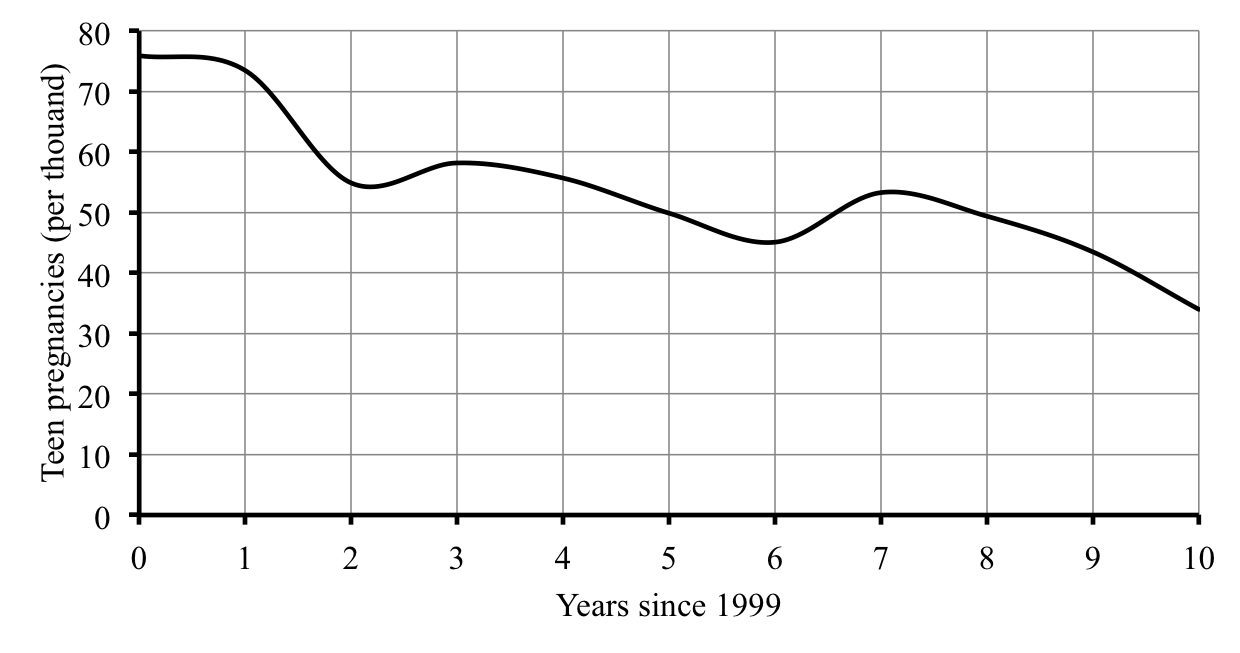
\includegraphics [width = 6in] {teenpregnancy.png}}
\end{center}
\begin{enumerate}
\item What was the teen pregnancy rate in 2003? \vfill
\item Did the teen pregnancy rate increase or decrease from 2003 to 2004? \vfill
\item While the teen pregnancy rate has generally decreased, from 2001 to 2002 it actually increased.  Were there other times when it increased?  \vfill
\item When did the teen pregnancy rate first fall below 60 pregnancies per thousand teens? \vfill
\item How fast was the teen pregnancy rate dropping on average per year from 2002 to 2005?  How does that compare to 2006 to 2009?   \vfill
\end{enumerate}

\end{enumerate}

\newpage


\noindent \textbf{When you're done \ldots}

\begin{itemize}
\item [$\Box$] Check your solutions.  Still confused?  Work with a classmate, instructor, or tutor.
\item [$\Box$] Try the \textbf{Do you know} questions.  Not sure?  Read the textbook and try again.
\item [$\Box$] Make a list of key ideas and process to remember under \textbf{Don't forget!}
\item [$\Box$] Do the textbook exercises and check your answers. Not sure if you are close enough? Compare answers with a classmate or ask your instructor or tutor.  
\item [$\Box$] Getting the wrong answers or stuck?  Re-read the section and try again.   If you are still stuck, work with a classmate or go to your instructor's office hours or tutor hours.
\item [$\Box$] It is normal to find some parts of exercises difficult, but if most of them are a struggle, meet with your instructor or advisor about possible strategies or support services.
\end{itemize}





\bigskip

\noindent \textbf{Do you know \ldots} %Rate of change

\begin{enumerate} [(a)]
\item How to calculate rate of change between two points?   \emph{Ask your instructor if you need to remember the formula or if it will be provided during the exam.} 
\item What the rate of change means in the story?   
\item How we can use the rate of change to estimate values?   
\item When a function is increasing or decreasing, and the connection to the rate of change?   
\item Why the rate of change is zero at the maximum (or minimum) value of a function?   
\item What the connection is between rate of change and the steepness of the graph?  
\end{enumerate}

\bigskip

\noindent \textbf{Don't forget!}


